\documentclass[10pt,twoside]{article}
\usepackage[utf8]{inputenc}
\usepackage{amsmath}
\usepackage{amsfonts}
\usepackage{amssymb}
\usepackage[spanish,es-noshorthands]{babel}
\usepackage[T1]{fontenc}
\usepackage{lmodern}
\usepackage{graphicx,hyperref}
\usepackage{tikz,pgf}
\usepackage{marvosym}
\usepackage{multicol}
\usepackage{subfig}
\usepackage[papersize={8.5in,13in},top=1.5cm,bottom=1.25cm,left=1cm,right=1cm]{geometry}
\usepackage{fancyhdr}
\pagestyle{fancy}
\fancyhead[LE]{Colegio Arborizadora Baja}
\fancyhead[RE]{PEI:``Hacia una cultura para el desarrollo sostenible''}
\fancyfoot[RO]{\Email gavendanor@colarborizadorabaja.edu.co}
\fancyhead[LO]{\url{www.colarborizadorabaja.edu.co}}
\fancyfoot[RE]{\Email cedarborizadoraba19@redp.edu.co}
\fancyfoot[LE]{Calle 59I \#44A - 02 \Telefon 7313994 - 7313995}
\fancyhead[RO]{Nit 830024976-8, Código DANE 11100103084-8}

\author{Germ\'an Avenda\~no Ram\'irez~\thanks{Lic. Mat. U.D., M.Sc. U.N.}}
\title{\begin{minipage}{.2\textwidth}

\includegraphics[height=1.75cm]{Images/logo-colegio.png}\end{minipage}
\begin{minipage}{.55\textwidth}
\begin{center}
Gestión del Riesgo\\
Plan Lector Ciclo IV
\end{center}
\end{minipage}\hfill
\begin{minipage}{.2\textwidth}

\includegraphics[height=1.75cm]{Images/logo-sed.png} 
\end{minipage}}
\date{}
\begin{document}
\maketitle
\begin{multicols}{2}
Haga la siguiente lectura cuidadosamente.
\section*{Amenaza sísmica en Bogotá, ¿mito o realidad?\footnote{Extracto de un artículo de Cristina Dimaté
PhD en Física Profesora Departamento de Geociencias Universidad Nacional Bogotá y de Mónica Arcila Geóloga Profesional Especializado Red Sismológica de Colombia-Ingeominas}}
Con relativa frecuencia se nos ha advertido que un sismo no se puede evitar, pero si la forma en que tu puedes reaccionar ante un evento de esta naturaleza. A los bogotanos nos sorprende, especialmente a los más jóvenes de que un sismo realmente pueda ocurrir. El máximo contacto que han tenido los habitantes en la últimas décadas con los sismos en la ciudad fue un moderado remezón en enero de 1999, cuando ocurrió el sismo que destruyó buena parte de Armenia y varios municipios del Eje Cafetero. Los \emph{jóvenes} de los años sesenta recuerdan algo más fuerte: en febrero de 1967, cuando un sismo con epicentro en el norte de Huila originó un fuerte movimiento del suelo en Bogotá, causó pánico y nos obligó a salir corriendo de las escuelas, colegios, trabajos, hogares, etc. En esa ocasión hubo en la ciudad 13 muertos, cerca de 100 heridos, se cayeron muros de varios lotes, hubo averías más o menos serias en 30 inmuebles, incluyendo bancos, colegios, varias casas antiguas de dos pisos, edificios de propiedad horizontal e iglesias (Ramírez, 1975: 205-206).

Afortunadamente, los grandes sismos son eventos raros, al menos
en nuestra percepción de tiempo de la vida cotidiana. Por ello, en Colombia, a pesar de que la mayor parte de nuestra población habita en zonas de amenaza sísmica alta o intermedia (Bogotá en
esta última), un bajo porcentaje puede afirmar que ha sido afectado de manera grave por un sismo. Como los sismos ocurren con poca frecuencia, el estudio de la amenaza sísmica requiere el concurso de varias disciplinas para develar patrones de ocurrencia y de cómo afecta a la naturaleza: geólogos, que buscan e interpretan las huellas que han dejado en el paisaje las rupturas de la corteza terrestre que han ocurrido en los últimos miles de años; historiadores, que recuperan los relatos de los habitantes
sobre los eventos que los afectaron fuertemente y ameritan un registro escrito u oral; sismólogos, que indagan los detalles de la fractura en el espacio y en el tiempo; ingenieros, que estudian el comportamiento de los suelos y estructuras ante las ondas sísmicas, etc. Como resultado de investigaciones de este tipo que se han realizado en el país, hoy podemos plantear hipótesis
sobre la posible ocurrencia de un evento sísmico que puede afectar de manera importante a Bogotá.
\subsection*{¿Por qué se producen los sismos? ¿Con qué frecuencia ocurren?}
Los sismos ocurren cuando la energía de deformación, que se ha acumulado durante mucho tiempo en las gigantescas masas de roca que conforman la corteza terrestre, se libera súbitamente ocasionando fractura y movimiento relativo entre las partes. En este proceso se generan ondas sísmicas que se propagan a través de la corteza a grandes distancias. Este fenómeno se produce principalmente a lo largo de fallas geológicas, que son zonas de debilidad de la corteza, relativamente estrechas, a lo largo de las cuales las masas de roca se deslizan entre sí. Esas zonas donde se ha detectado que hay movimiento relativo en el presente se denominan fallas activas.

La frecuencia con que suceden los sismos de una magnitud dada se expresa a través de la relación de Gutenberg-Richter:
\[\log(N)=a+bM\]
donde $N$ es el número acumulado de sismos con magnitud mayor a $M$ que ocurren en un área especificada y en un tiempo, y $a$ y $b$ son constantes que varían de región en región. Un análisis del catálogo colombiano muestra que en promedio en nuestro país ocurre
un sismo de magnitud mayor a 6.0 por año. Esto, incluyendo los eventos que ocurren costa afuera, en el Océano Pacífico, y los de profundidad mayor a 100 km, los cuales no percibimos porque el
movimiento que causan en la superficie es pequeño.
\subsection*{Sismos históricos que han afectado a Bogotá}
El mejor testimonio de la historia sísmica de Bogotá, como lo escribe Ramírez, es la iglesia del cerro de Guadalupe
\begin{quote}
\textit{La ermita de Guadalupe, en el cerro de su nombre en Bogotá, se
fundó en 1656 (...) El terremoto de 1743 la destruyó por primera vez (...) La ermita se reconstruyó en 1760, y volvió a arruinarse en el terremoto de 1785. Reconstruida, la derribó el sacudimiento telúrico de 1827, para ser reconstruida de nuevo y volver a tierra
en los temblores de Bogotá de 1917. El templo, que hoy se llama Guadalupe, con su bella estatua, data de los últimos 30 años, y es de una construcción más sólida. Sin embargo, la imagen de
la Virgen que adornaba la fachada se fragmentó en el antebrazo y el hombro derecho durante el terremoto del Huila del 9 de febrero de 1967 (Ramírez, 1975: 78).}
\end{quote}
Por lo menos seis eventos bien documentados han causado daños
significativos en la ciudad durante los últimos 270 años: los sismos de 1743, 1785, 1826, 1827, 1917 y 1967.

El sismo del 18 de octubre de 1743 causó sus mayores daños en la Provincia de Oriente en Cundinamarca (Fómeque, Cáqueza, Fosca, etc.) y también en Bogotá. Según documentos del Archivo
Nacional citados por Ramírez (Ramírez, 1975: 77-78): “... causándose en esta ciudad ruinas tan notables que raras casas
del lugar dejaron de padecerlas...”. Además del templo de Guadalupe, “... en los demás templos y conventos se han experimentado dichas ruinas, como se manifestó en los de San Agustín, San Francisco, Egipto, el Carmen y las Cruces, (...) siendo el daño que experimentaron dichos conventos gravísimo”.
\subsection*{El sismo de 1917}
El 31 de agosto de 1917, a las 6:30 de la mañana, un fuerte terremoto prácticamente destruyó Villavicencio y causó graves daños en San Martín, Fosca, Cáqueza, Colonia y varias poblaciones aledañas (Sanabria y Cifuentes, 2005). Los destrozos fueron tan graves que se contempló la posibilidad de reconstruir Villavicencio en otro lugar. La intensidad de los daños, los reportes de deslizamientos y la continuidad de las réplicas sentidas por la población en estos lugares indican que el epicentro del sismo se localizó posiblemente hacia el flanco oriental de la Cordillera Oriental entre Villavicencio y San Martín. Aun fuera de la zona epicentral, muchas poblaciones sufrieron también daños: Fusagasuga, Ibagué, Espinal, Fresno, Mariquita, Pensilvania, por ejemplo, y por supuesto Bogotá, Soacha, Madrid, Facatativá, entre otras, en la Sabana.

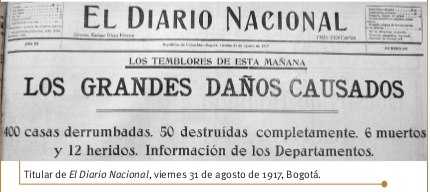
\includegraphics[scale=.56]{Images/Pantallazo51.png} 

En Bogotá los daños fueron significativos y agravados por un sismo el día anterior y por varias réplicas fuertes que siguieron al sismo principal. El Diario Nacional del 31 de agosto de 1917 informa así lo que se percibía en la ciudad:
\begin{quote}
\textit{A las 7 menos 25 minutos de la mañana se verificó el nuevo temblor de duración e intensidad muy superiores a los de la noche anterior. Fue una convulsión trágica y macabra que hizo bambolear los edificios de Bogotá. Los habitantes angustiados se salieron a las calles, nuevamente llenos de pánico y angustia; y allí
comenzó a salir cuán numerosos habían sido los daños que el espantoso cataclismo había causado y cuánta gravedad revestían. Podemos asegurar que no hay una sola casa de verdad que no sufriera algún daño; igualmente puede comprenderse que si se repite un nuevo temblor, la mayoría de las casas se derrumbarán. El enorme pánico que hay en toda la ciudad no puede ser,
pues, injustificado.}
\end{quote}
En el mismo periódico un reporte de la Policía Nacional da cuenta de 400 casas derrumbadas, 50 destruidas completamente, seis muertos y 12 heridos (fotos 1, 2 y 3). Daños importantes sufrieron edificios como la catedral, la iglesia de Chapinero, que perdió su torre principal, el claustro de Nuestra Señora del Rosario, el hospital San Juan de Dios, el Palacio Liévano y otros edificios gubernamentales y bastantes residencias privadas. La total destrucción de casas solamente ocurrió en algunos pocos casos.
\subsection*{Bibliografía}
Ramírez, J. E. (1975), Historia de los terremotos en Colombia, segunda edición, Bogotá, Instituto Geográfico Agustín Codazzi, Subdirección de Investigaciones y Divulgación Geográfica

Sanabria, A. M. y Cifuentes, H. G. (2005), Análisis histórico-geográfico de los sismos ocurridos en 1785 y 1917 para la determinación de epicentros e intensidades, trabajo de grado, Bogotá, Facultad de Ciencias Humanas, Departamento de Geografía, Universidad Nacional de Colombia.
\section*{Actividad 1}
Responda a las siguientes preguntas sobre la lectura en una hoja anexa.
\begin{enumerate}
\item ¿Cuál ha sido el sismo más fuerte que hayamos sentido los habitantes de la capital en las dos últimas décadas?
\item ¿En qué parte de Colombia fué el epicentro del sismo de 1967 que se sintió fuerte en Bogotá?
\item Se considera que Bogotá está en una zona de amenaza sísmica
\begin{enumerate}
\begin{multicols}{3}
\item ¿Alta?
\item ¿Media?
\item ¿Baja?
\end{multicols}
\end{enumerate}
\item ¿Cuál ha sido el más fuerte sismo que se ha presentado en Bogotá en los últimos 200 años?
\item ¿Qué profesionales se dedican o se necesitan para estudiar la amenaza sísmica y qué hace cada uno de ellos al respecto?
\item ¿Se puede plantear una hipótesis con los datos conocidos sobre la posibilidad de un sismo en Bogotá?
\item ¿Por qué se producen los sismos?
\item ¿Con qué frecuencia ocurren los sismos?
\item ¿Con qué frecuencia ocurren los sismos con una magnitud mayor o igual a 6.0 en nuestro país?
\item ¿Cuántas veces ha sido destruída la ermita de Guadalupe?
\item Enumere los principales sismos que se han sentido  en Bogotá durante los últimos 270 años.
\item ¿Dónde fue el epicentro del sismo que afectó a Bogotá en 1917?
\item Haga una breve síntesis del
\end{enumerate}
\section*{Qué hacer frente a un posible sismo que afecte nuestra ciudad?}
Como sabemos ya, no se puede predecir exacamente cuando ocurrirá un sismo, sin embargo si podemos prepararnos ante cualquier emergencia que pueda suceder. Para éstos debemos tener en cuenta las siguiente pautas.
\begin{enumerate}
\item \textbf{Informarnos}: Debemos informarnos de cuáles son los posibles elementos que pueden aumentar el nivel de riesgo frente a un posible sismo que nos afecte. He aquí algunas recomendaciones
\begin{enumerate}
\item Asegura o cambia de lugar los objetos que se pueden mover, caer y hacerte daño.
\item Elimina fuente potenciales de incendio.
\end{enumerate}
\item \textbf{Preparanos}: Debemos prepararnos y para ello, debemos establecer acuerdos sobre como reaccionar frente a una emergencia. Aquí algunas recomendaciones
\begin{enumerate}
\item Establecer acuerdos sobre como actuar frente a un posible sismo o emergencia. Se deben establecer las rutas de evacuación y la ubicación de sitios seguros para los puntos de encuentro.
\item Tener un kit que nos permita sobrevivir por 72 horas.
\item Identificar formas de autoprotección
\item Participar activamente de los simulacros que se programen.
\end{enumerate}
\end{enumerate}
\section*{Actividad 2}
\begin{enumerate}
\item Identifique que objetos pueden representar un peligro en la institución.
\item Describa la señalización de las rutas de evacuación en el colegio.
\item Haga un mapa de la ruta de evacuación que debería seguir en caso de emergencia para llegar al punto de encuentro.
\item Haga un listado de los recursos que usted conoce del equipo (kit) que puede ser útil en caso de emergencia.
\item Invente un logotipo que represente el Plan de Gestión de Riesgo 2017.
\end{enumerate}
\end{multicols}
\end{document}
